
    \documentclass[a4paper, twoside, russian, ngerman]{book}%[a4paper,oneside] ngerman für "=
    \usepackage[pass]{geometry}%[hmarginratio=1:1]{geometry}
    \usepackage{makeidx}
    \usepackage{amsmath}
    \usepackage{amssymb}
    \usepackage{mathabx}
    \usepackage{csquotes}
    \usepackage{afterpage}
    \usepackage{xcolor}
    \usepackage{tikz}
    \usetikzlibrary{shapes,backgrounds,arrows,calc,positioning}
    \usetikzlibrary{calendar,fpu}
    
    \usepackage{ifthen}
    \usepackage{intcalc}
    
    \usepackage[citecolor=black,urlcolor=black,linkcolor=black,breaklinks=true]{hyperref}
    \hypersetup{
        colorlinks=true
    }
    \usepackage{datetime2}
    
    \usepackage[xindy={language=english,codepage=duden-utf8},
        nonumberlist,
        toc,
        nopostdot,
        style=altlist,
        nogroupskip
        ]{glossaries}
        \GlsSetXdyCodePage{duden-utf8}
    \apptocmd{\thebibliography}{\raggedright}{}{}
    
    
    \usepackage{fontspec}
    \setromanfont{CMU Serif}
    \setsansfont{CMU Sans Serif}
    \setmonofont{CMU Typewriter Text}

    
    \begin{document}

    \newcommand{\coverLineA}{\huge \textbf{Umbratica}}
\newcommand{\coverLineB}{\normalsize \textbf{\DTMnow}}

\begin{titlepage}
    \begin{tikzpicture}[remember picture,overlay,shift={(current page.south west)}]

        %\node[shape=rectangle, fill=white, minimum width=\paperwidth, minimum height=\paperheight] at (current page.center) {};
        \node[inner sep=0pt] at (current page.center) {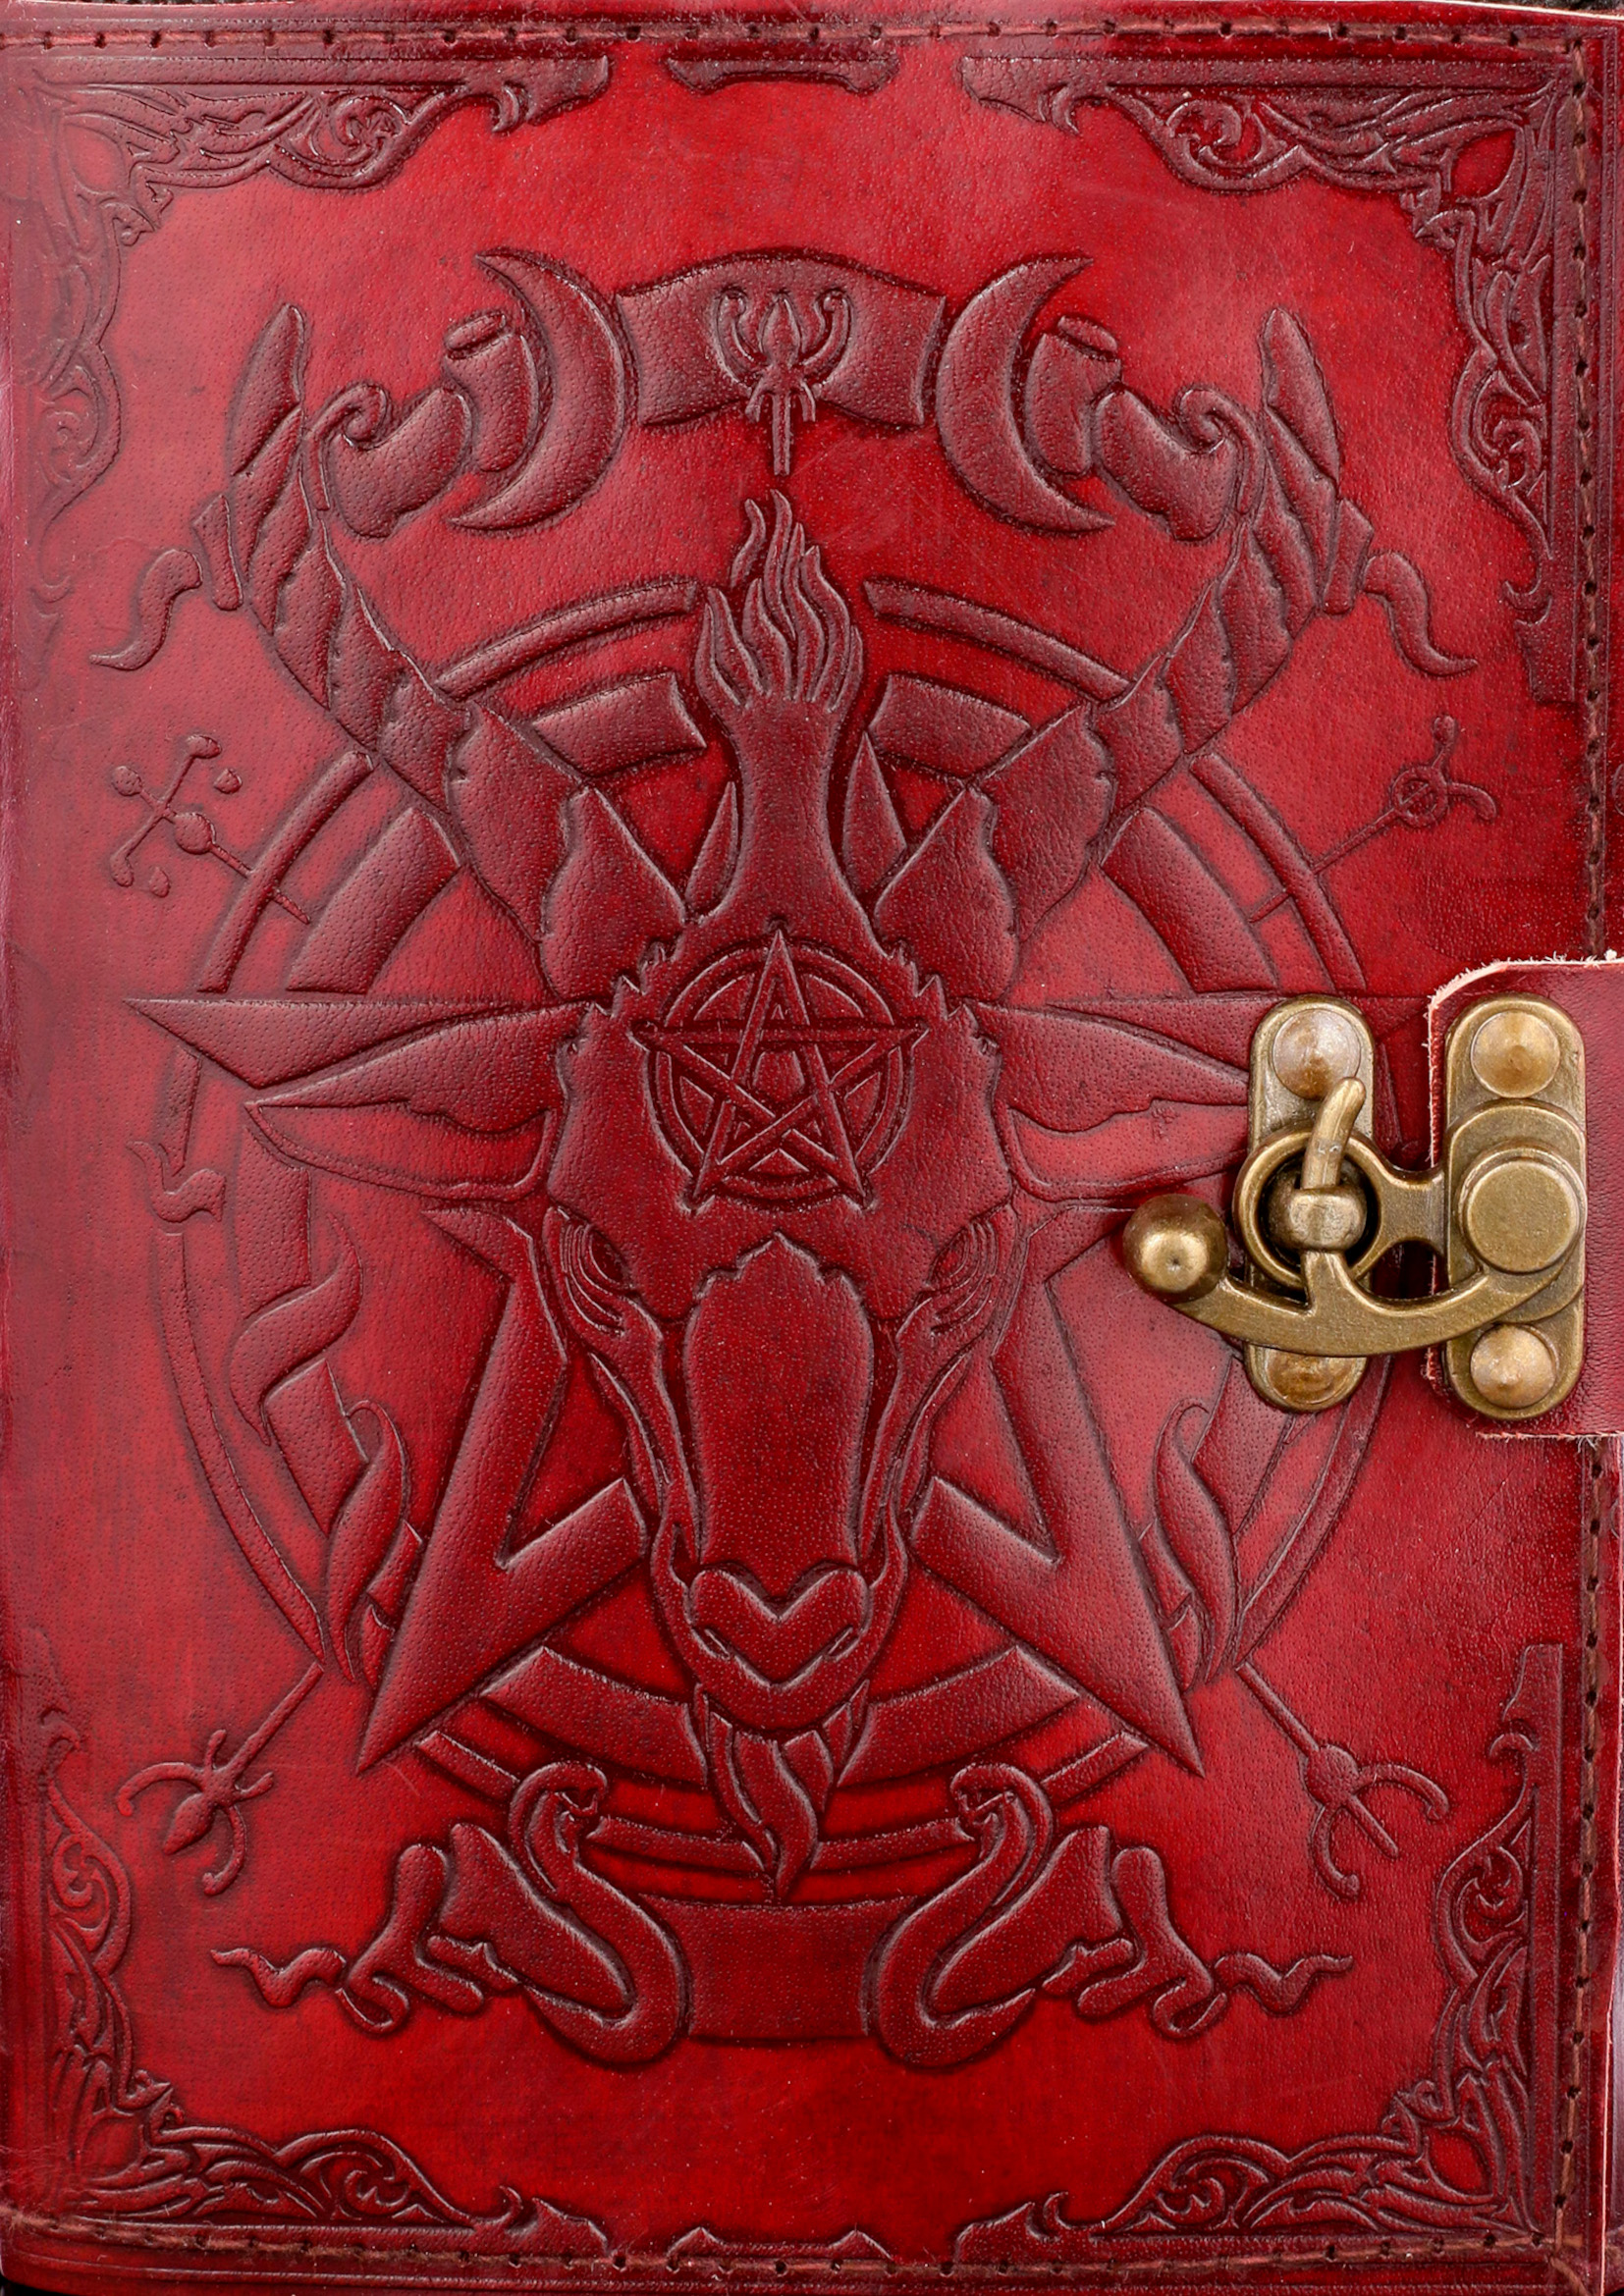
\includegraphics[width=\paperwidth,height=\paperheight]{img/cover.jpg}};
        \node[inner sep=0pt, text=red!20!black] at ($(current page.south)+(-0.01,1.29cm)$) {\coverLineA};
        \node[inner sep=0pt, text=red!60!black] at ($(current page.south)+(0.005,1.305cm)$) {\coverLineA};
        \node[inner sep=0pt, text=red!40!black] at ($(current page.south)+(0,1.3cm)$) {\coverLineA};
        \node[inner sep=0pt, text=red!20!black] at ($(current page.south)+(-0.01,0.49cm)$) {\coverLineB};
        \node[inner sep=0pt, text=red!60!black] at ($(current page.south)+(0.005,0.505cm)$) {\coverLineB};
        \node[inner sep=0pt, text=red!40!black] at ($(current page.south)+(0,0.5cm)$) {\coverLineB};

    \end{tikzpicture}
\end{titlepage}


    \setlength{\parskip}{1ex}
    
    In the year...
    
    \end{document}
    